\documentclass[conference]{IEEEtran}
\IEEEoverridecommandlockouts

\usepackage{cite}
\usepackage{amsmath,amssymb,amsfonts}
\usepackage{algorithmic}
\usepackage{graphicx}
\usepackage{textcomp}
\usepackage{xcolor}
\usepackage{hyperref}
\def\BibTeX{{\rm B\kern-.05em{\sc i\kern-.025em b}\kern-.08em
T\kern-.1667em\lower.7ex\hbox{E}\kern-.125emX}}

\begin{document}

    \title{Cross-Platform Quantum Compiler for Synthesizing Quantum Circuits Based on Arbitrary Hamiltonians \\
    \thanks{This work was supported in part by personal funding and community feedback.}
    }

    \author{\IEEEauthorblockN{Shoupu Wan}
    \IEEEauthorblockA{\textit{Independent Researcher} \\
    \textit{Quantum Compiler Project}\\
    United States \\
    wanshoupu@gmail.com}
    }

    \maketitle

    \begin{abstract}
        Quantum software development is challenged by hardware heterogeneity and the lack of unified compilation frameworks.
        We present a versatile quantum compiler designed to decompose arbitrary Hamiltonians into quantum circuits expressed via a platform-independent intermediate language (IL).
        This IL serves as a universal representation, enabling flexible translation and optimization across diverse quantum hardware backends.
        We also present designs of renderers to convert the IL into executable quantum circuits into the target quantum computing platforms such as Qiskit and Cirq.
    \end{abstract}

    \begin{IEEEkeywords}
        Quantum Computing, Quantum Compilation, Hamiltonian Decomposition, Cross-Platform, Circuit Synthesis, Solovay-Kitaev Theorem,
    \end{IEEEkeywords}


    \section{Introduction}\label{sec:introduction}

    Quantum software development today is hindered by fragmentation arising from diverse hardware architectures and incompatible compiler toolchains.
    Developers often resort to writing custom code tailored for each quantum software development kit (SDK) such as Qiskit, Cirq, or Braket,
    limiting portability and increasing development overhead.
    To address this challenge, we present a cross-platform quantum compiler that takes a user-defined Hamiltonian as input and produces optimized quantum
    circuits executable across multiple hardware platforms.
    Our compilation framework employs a multi-stage decomposition strategy—including two-level decomposition (2L),
    Swap gate decomposition (CX), control decomposition (CTRL), Euler angle decomposition (ED), and Solovay-Kitaev approximation (SK)—to systematically
    translate high-level Hamiltonians into gate-level instructions~\cite{nielsen2010quantum}.
    The compiler offers a high degree of configurability, enabling tiered optimization strategies and fine-grained control over decomposition granularity.
    This flexibility allows tailoring the output circuits to the unique constraints and capabilities of different quantum hardware architectures,
    thereby maximizing efficiency and portability.
    Currently, our compiler supports popular platforms such as Qiskit and Cirq, with ongoing development to extend to additional frameworks including AWS Braket and PennyLane.


    \section{Motivation}\label{sec:motivation}

    The field of quantum computing is advancing rapidly, but software development remains fragmented
    due to the lack of standardized workflows across quantum platforms.
    Each hardware vendor or software framework often promotes its own SDK and compiler infrastructure,
    creating silos that hinder collaboration, reproducibility, and long-term sustainability.
    This fragmentation poses several challenges: researchers must rewrite or reoptimize circuits for each backend,
    making it difficult to compare results or share code.
    Educational materials and benchmarks tied to a specific toolchain may not translate to others, slowing down learning and adoption.
    Furthermore, the fast-evolving nature of quantum hardware leads to shifting gate sets and constraints,
    exacerbating incompatibility issues.
    Existing toolchains often lock users into proprietary ecosystems, limiting flexibility and cross-platform experimentation.
    As a result, developers face unnecessary barriers when exploring algorithm performance across different quantum processors or
    when trying to integrate novel decomposition techniques into existing stacks.
    To address these limitations, we introduce a cross-platform quantum compiler that decouples high-level algorithm design
    from hardware-specific implementation details.
    By promoting abstraction through a common intermediate representation, our compiler enables code portability,
    encourages reproducible workflows, and accelerates the prototyping of quantum algorithms across diverse environments.


    \section{Method}\label{sec:method}

    Given an input Hamiltonian $H = \sum_j c_j P_j$ expressed as a linear combination of Pauli strings,
    we decompose $H$ using operator synthesis techniques and compile it into gate-level circuits.
    The compiler backend maps circuits into native gates for Qiskit, Cirq, or other selected platforms.
    Users can toggle basis sets and optimization levels.


    The compilation process proceeds in two primary stages: **operator decomposition** and **platform-specific gate synthesis**.

    \subsection{Operator Decomposition}\label{subsec:operator-decomposition}
    Each exponential term of the form $e^{-i c_j P_j t}$ must be translated into a quantum circuit.
    Our compiler uses a configurable pipeline of operator synthesis techniques to achieve this translation.
    The supported decomposition strategies include:

    \begin{itemize}
        \item{\textbf{Two-Level Decomposition (2L):} Breaks down multi-qubit unitaries into elementary 2-level operations.}
        \item{\textbf{Swap Decomposition (CX):} Rewrites circuits with long-range qubit interactions into topologies
        with nearest-neighbor constraints using SWAP and CNOT gates.}
        \item{\textbf{Control Decomposition (CTRL):} Decomposes controlled unitaries, preserving
        the structure of controlled operations in gate-level terms.}
        \item{\textbf{Euler Decomposition (ED):} Converts arbitrary single-qubit unitaries into a minimal sequence of rotations
        from a chosen basis (e.g., Z-Y-Z).}
        \item{\textbf{Solovay-Kitaev Approximation (SK):} Approximates arbitrary unitaries with sequences over a finite universal gate set,
            useful when target hardware supports only limited gates.}
    \end{itemize}

    These decomposition steps can be selectively enabled or ordered based on the user’s preferences and the constraints of the target hardware.

    \subsection{Platform-Specific Backend Translation}\label{subsec:platform-specific-backend-translation}
    Once the IL (intermediate language) circuit is constructed, it is passed to a backend-specific renderer that maps it into native gates supported by the desired quantum SDK—currently Qiskit or Cirq. Backend renderers are modular and support:

    \begin{itemize}
        \item Selection of the target gate basis (e.g., \{\texttt{X}, \texttt{Y}, \texttt{Z}, \texttt{H}, \texttt{CX}\} for IBM Q).
        \item Application of transpiler passes, such as gate fusion, qubit routing, or noise-aware optimization.
        \item Export of executable code in a form that can be directly submitted to hardware or simulators.
    \end{itemize}

    Users can configure optimization levels, toggle specific synthesis techniques, and specify target constraints such as qubit connectivity or native gate sets.

    This modular design ensures that the compiler remains extensible and adaptable to future hardware changes and supports integration with additional platforms such as PennyLane, Braket, and beyond.

    \subsection{Gate Translation Pipeline}\label{subsec:gate-translation-pipeline}
    Each Pauli term is individually mapped via exponentiation: $e^{-iHt} \approx \prod_j e^{-ic_j P_j t}$.
    Our pipeline then:
    \begin{enumerate}
        \item Translates Pauli exponentials into native gate sequences.
        \item Applies platform-specific transpilation.
        \item Outputs backend-executable code with minimal overhead.
    \end{enumerate}

    \subsection{Example Output}\label{subsec:example-output}
    \begin{figure}[htbp]
        \centerline{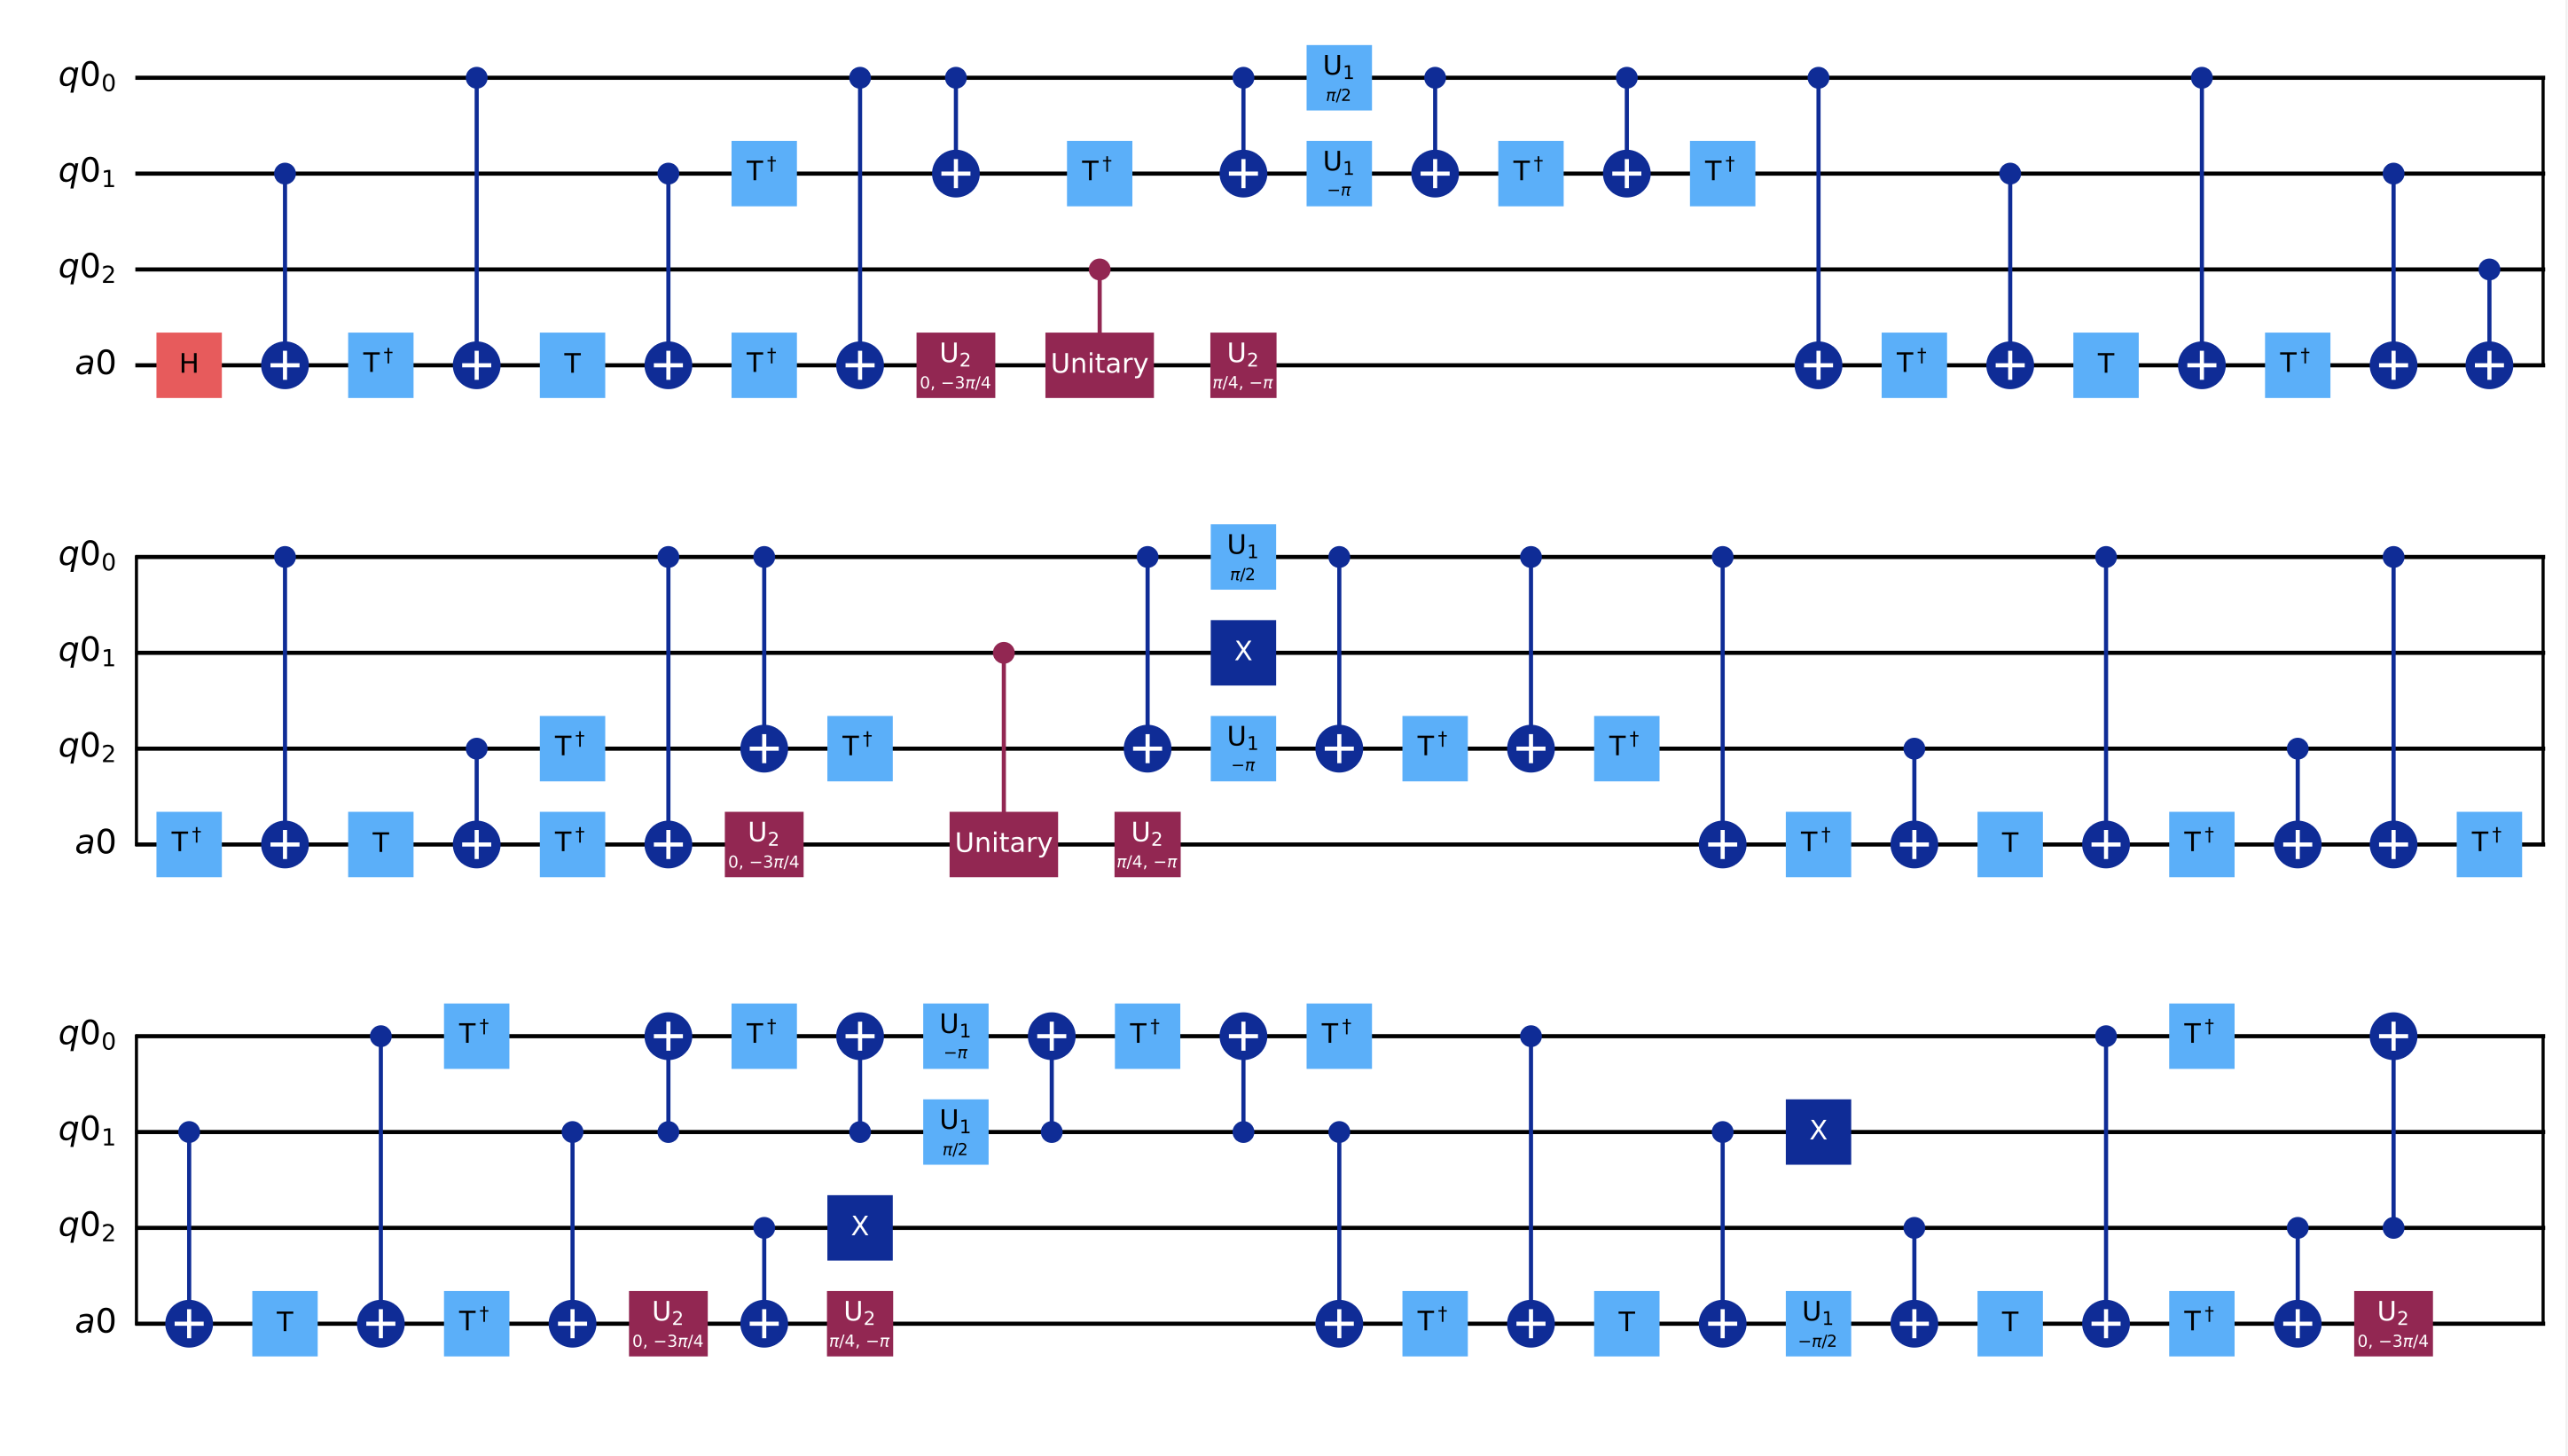
\includegraphics[width=0.45\textwidth]{circuit-example}}
        \caption{Compiled circuit from a 2-qubit Heisenberg model in Cirq and Qiskit.}
        \label{fig:compiled-circuit}
    \end{figure}


    \section{Results}\label{sec:results}
    Initial benchmarks show the compiler produces correct circuits consistent across backends,
    demonstrating the compiler’s potential to simplify quantum algorithm development and
    accelerate experimentation in heterogeneous quantum computing environments.


    \section{Conclusion and Future Work}\label{sec:conclusion-and-future-work}
    This project reduces platform friction in quantum software development.
    Future work includes:
    \begin{itemize}
        \item Integrating PennyLane and AWS Braket support
        \item Adding classical-quantum hybrid workflows
        \item Implementing circuit equivalence checking
    \end{itemize}
    We invite collaboration and feedback from the quantum software community.

    \begin{thebibliography}{00}
        \bibitem{nielsen2010quantum}
        M. A. Nielsen and I. L. Chuang, \textit{Quantum Computation and Quantum Information}, Cambridge Univ. Press, 2010.

        \bibitem{dawson2005solovaykitaevalgorithm}
        C. M. Dawson and M. A. Nielsen, “The Solovay-Kitaev algorithm,”
        arXiv preprint quant-ph/0505030, 2005. [Online]. Available: \url{https://arxiv.org/abs/quant-ph/0505030}

        \bibitem{qiskit2023}
        H. Abraham, AduOffei, I. Y. Akhalwaya, et al.,
        “Qiskit: An open-source framework for quantum computing,”
        \textit{Zenodo}, 2023. doi: 10.5281/zenodo.2562111.

        \bibitem{cirq2024}
        Google Quantum AI, “Cirq,” 2024. [Online]. Available: \url{https://quantumai.google/cirq}
    \end{thebibliography}

\end{document}
